%==============================================================================
% ETHASL - Template for student projects at the ASL
% 2013.10: Péter Fankhauser
% This template is based on the IMRT Latex template by Eric A. Mueller.
%==============================================================================

\documentclass[10pt,twoside,a4paper]{report}

\usepackage{pdfpages}

% ETHASL package
% TODO Choose options according to your project
% som/bt/st/mt: Studies on Mechatronics, Bachelor Thesis, Semester Thesis, Master Thesis
% fs/hs: Spring term, Autumn term
% german/english: German/English
\usepackage[bt,hs,english]{packages/ethasl}

% Activate for german language
%\usepackage{german}
%\usepackage{ae}

% Graphics
\usepackage{graphicx}
\graphicspath{ {./images/} }

%%%%%%%%%%%%%%%%%%%%%%%%%%%%%%%%%%%%%%%%%%%%%%%%%%%%%%%%%%%%%%%%%%%%%%%%%%%%%%%
% LaTeX preamble
%%%%%%%%%%%%%%%%%%%%%%%%%%%%%%%%%%%%%%%%%%%%%%%%%%%%%%%%%%%%%%%%%%%%%%%%%%%%%%%
% Encoding settings
\usepackage[utf8]{inputenc}
\usepackage[OT1]{fontenc}

% Paper size
\usepackage{a4}

% Headings
\usepackage{fancyhdr}

% More symbols
\usepackage{textcomp}\usepackage{gensymb}

% Math support for Times font
%\usepackage{txfonts}

% ISO date
\usepackage[english]{isodate}

% Multi column
\usepackage{multicol}

% Figures
\usepackage{graphicx}

% Subfigures (obsolete)
\usepackage{subfigure}

% Bibliography
\usepackage[numbers]{natbib}

% Nicer tables
\usepackage{booktabs}
\usepackage{array}
\usepackage{multirow}

% Colors
\usepackage{color}
\usepackage{colortbl}
\definecolor{black}{rgb}{0,0,0}
\definecolor{white}{rgb}{1,1,1}
\definecolor{darkred}{rgb}{0.5,0,0}
\definecolor{darkgreen}{rgb}{0,0.5,0}
\definecolor{darkblue}{rgb}{0,0,0.5}

% Additional math functionality
\usepackage{amsmath}
\usepackage{amssymb}

% Nice fractions
\usepackage{nicefrac}

% Upper case greek letters
\usepackage{upgreek}

% ISO math notation
\usepackage{isomath}
\renewcommand{\vec}{\vectorsym}
\newcommand{\mat}{\matrixsym}

% Units
\usepackage{units}

% Rotated objects
\usepackage{rotating}

% Indent
\setlength{\parindent}{0em}

% Include PDF pages
\usepackage{pdfpages}
\includepdfset{pages={-}, frame=true, pagecommand={\thispagestyle{fancy}}}

% Headings
\rhead[\thepage]{\nouppercase{\rightmark}}
\lhead[\nouppercase{\leftmark}]{\thepage}
\cfoot{}

% Gantt chart
\usepackage{pgfgantt}

% Links (last package)
\PassOptionsToPackage{hyphens}{url}\usepackage{hyperref}

% Clever references (has to be loaded after hyperref)
\usepackage{cleveref}


%%%%%%%%%%%%%%%%%%%%%%%%%%%%%%%%%%%%%%%%%%%%%%%%%%%%%%%%%%%%%%%%%%%%%%%%%%%%%%%
% Title page
%%%%%%%%%%%%%%%%%%%%%%%%%%%%%%%%%%%%%%%%%%%%%%%%%%%%%%%%%%%%%%%%%%%%%%%%%%%%%%%
\begin{document}

\title{Unified Path Following for Hybrid VTOLs}
%\subtitle{bla bla bla}

% TODO Add name of the authors
\studentA{Junwoo Hwang}

% TODO Add name of the supervisors
\supervisionA{Jaeyoung Lim}
\supervisionB{Florian Achermann}
\supervisionC{David Rohr}

% TODO Change if necessary
\projectYear{\the\year} % This year
%\projectYear{\advance\year by -1 \the\year\advance\year by 1} % Last year

\maketitle
\pagestyle{plain}
\pagenumbering{roman}

%%%%%%%%%%%%%%%%%%%%%%%%%%%%%%%%%%%%%%%%%%%%%%%%%%%%%%%%%%%%%%%%%%%%%%%%%%%%%%%
% Declaration of originality
%%%%%%%%%%%%%%%%%%%%%%%%%%%%%%%%%%%%%%%%%%%%%%%%%%%%%%%%%%%%%%%%%%%%%%%%%%%%%%%
% \pagestyle{empty}
% TODO Modify placeholders in declaration.tex
%% TODO Add title, student first/last name, supervisor first/last name.

\section*{Declaration of Originality}

\vspace{1cm}

I hereby declare that the written work I have submitted entitled

\vspace{0.5cm}

% TODO Add title
\textbf{Your Project Title}

\vspace{0.5cm}

is original work which I alone have authored and which is written in my own words.\footnote{Co-authored work: The signatures of all authors are required. Each signature attests to the originality of the entire piece of written work in its final form.}

\vspace{1cm}

\textbf{Author(s)}

\vspace{0.5cm}

\begin{tabular}{ p{5cm} p{5cm} }
% TODO Add student first/last name
  First name & Last name \\
\end{tabular}

\vspace{0.5cm}

\textbf{Student supervisor(s)}

\vspace{0.5cm}

\begin{tabular}{ p{5cm} p{5cm} }
% TODO Add supervisor first/last name
  First name & Last name \\
\end{tabular}

\vspace{0.5cm}

\textbf{Supervising lecturer}

\vspace{0.5cm}

\begin{tabular}{ p{5cm} p{5cm} }
  Roland & Siegwart \\
\end{tabular}

\vspace{1cm}

With the signature I declare that I have been informed regarding normal academic citation rules and that I have read and understood the information on 'Citation etiquette' (\url{https://www.ethz.ch/content/dam/ethz/main/education/rechtliches-abschluesse/leistungskontrollen/plagiarism-citationetiquette.pdf}).
The citation conventions usual to the discipline in question here have been respected.

\vspace{0.5cm}

The above written work may be tested electronically for plagiarism.

\vspace{4cm}

\begin{tabular}{ p{5cm} p{1cm} p{5cm} }
  \cline{1-1} \cline{3-3}
  Place and date & & Signature \\
\end{tabular}


% 
\includepdf[pagecommand={}]{chapters/declaration-originality.pdf}


%%%%%%%%%%%%%%%%%%%%%%%%%%%%%%%%%%%%%%%%%%%%%%%%%%%%%%%%%%%%%%%%%%%%%%%%%%%%%%%
% Table on contents
%%%%%%%%%%%%%%%%%%%%%%%%%%%%%%%%%%%%%%%%%%%%%%%%%%%%%%%%%%%%%%%%%%%%%%%%%%%%%%%

% Table of Contents depth (TODO change if necessary)
\setcounter{tocdepth}{2}

\tableofcontents
\cleardoublepage

%%%%%%%%%%%%%%%%%%%%%%%%%%%%%%%%%%%%%%%%%%%%%%%%%%%%%%%%%%%%%%%%%%%%%%%%%%%%%%%
% Chapters standard
%%%%%%%%%%%%%%%%%%%%%%%%%%%%%%%%%%%%%%%%%%%%%%%%%%%%%%%%%%%%%%%%%%%%%%%%%%%%%%%
% \chapter*{Preface}
\addcontentsline{toc}{chapter}{Preface}

This thesis was written because ...
\cleardoublepage

% \chapter*{Abstract}
\addcontentsline{toc}{chapter}{Abstract}

With the advancement of low-cost electronics and UAV components, an interesting hybrid vehicle type so-called 'Hybrid VTOL' has been under the spotlight of academia and researchers' interest recently. Due to its versatility of utilizing both modes of operation from two distinct vehicle regimes: Multirotor and Fixed Wing, this breed of vehicle can fly further in an energy-efficient manner, meanwhile preserving the capability to launch and land in a small confined space when needed.

However, Hybrid VTOLs usually have a decoupled Path Following a control strategy depending on its mode of operation. Although this approach works in a practical sense, both of the control strategies fail to capture the overall flexibility of the system.

In this thesis, a new Vector Field based Path Following formulation is derived and shown for supporting both fixed-wing and multirotor modes of operation.
\cleardoublepage

% % Set title used in nomenclature library
\renewcommand{\nomname}{Symbols}

%% This code creates the groups
% -----------------------------------------
\renewcommand\nomgroup[1]{%
  \item[\bfseries
  \ifstrequal{#1}{V}{Vehicle constraints}{%
  \ifstrequal{#1}{P}{Path Following parameters}{%
  \ifstrequal{#1}{S}{Vehicle states}{}}}%
]}
% -----------------------------------------

\nomenclature[V]{$V_{min}$}{Minimum Speed Vehicle can achieve}
\nomenclature[V]{$V_{nom}$}{Nominal Speed Vehicle can achieve (cruise speed for Fixed Wing)}
\nomenclature[V]{$V_{max}$}{Maximum Speed vehicle can achieve}
\nomenclature[P]{$V_{path}$}{Desired speed on path}
\nomenclature[P]{$V_{approach}$}{Desired approaching speed orthogonal to the path}
\nomenclature[P]{$V_{ref}^{\parallel}$}{Target velocity component parallel to path}
\nomenclature[P]{$V_{ref}^{\perp}$}{Target velocity component orthogonal (towards) to path}
\nomenclature[P]{$e$}{Cross track error distance to the path}
\nomenclature[P]{$e_{b}$}{Track error boundary}
\nomenclature[P]{$t_{const}$}{Track error boundary time constant}
\nomenclature[P]{$\hat{t_p}$}{Unit tangent vector of the path segment}
\nomenclature[P]{$\overline{e}$}{Normalized track error}
\nomenclature[S]{$\lambda$}{Course over ground}
\nomenclature[S]{$\xi$}{Heading}

% Make nomenclature chapter
\printnomenclature
\label{sec:symbols}
\addcontentsline{toc}{chapter}{Symbols}

% Indices
\section*{Indices}
\begin{tabbing}
 \hspace*{1.6cm}  \= \kill
 $x$ \> x axis \\[0.5ex]
 $y$ \> y axis \\[0.5ex]
\end{tabbing}

% Acronyms
\section*{Acronyms and Abbreviations}
\begin{tabbing}
 \hspace*{1.6cm}  \= \kill
 ETH \> Eidgenössische Technische Hochschule \\[0.5ex]
 UAV \> Unmanned Aerial Vehicle \\[0.5ex]
\end{tabbing}
\cleardoublepage

%%%%%%%%%%%%%%%%%%%%%%%%%%%%%%%%%%%%%%%%%%%%%%%%%%%%%%%%%%%%%%%%%%%%%%%%%%%%%%%
% Chapters custom
%%%%%%%%%%%%%%%%%%%%%%%%%%%%%%%%%%%%%%%%%%%%%%%%%%%%%%%%%%%%%%%%%%%%%%%%%%%%%%%
\pagestyle{fancy}
\pagenumbering{arabic}

\chapter{Introduction}
\label{sec:introduction}

\section{Motivation}
Hybrid VTOLs are particularly interesting vehicle to study, which has an intermediate mode as either a Multirotor, or a Fixed Wing.

\begin{figure}[h]
\centering
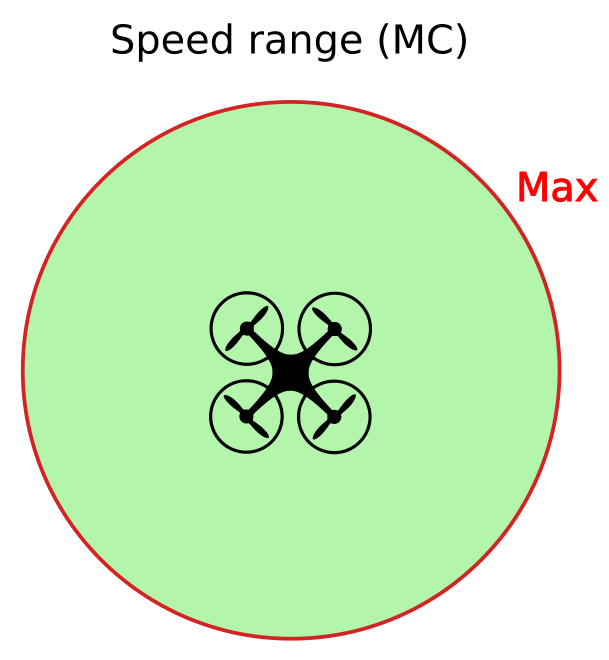
\includegraphics[width=0.3\textwidth]{MC_Velocity_Range}
\caption{Multirotor velocity range}
\end{figure}

\begin{figure}[h]
\centering
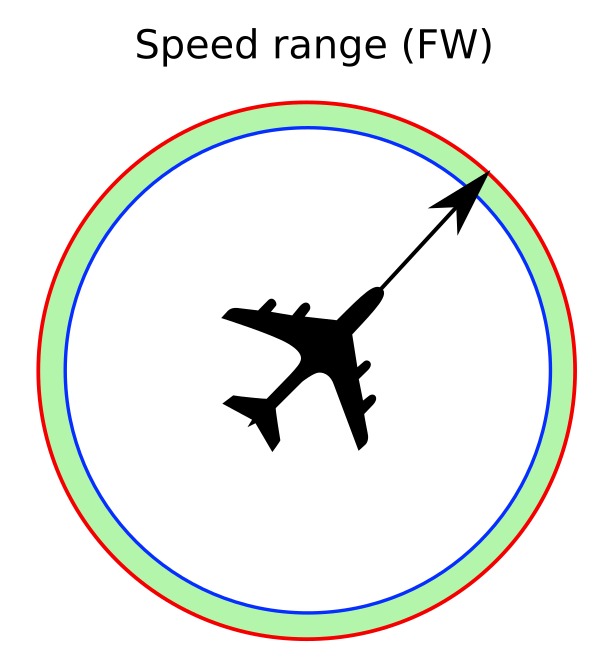
\includegraphics[width=0.3\textwidth]{FW_Velocity_Range}
\caption{Fixed Wing velocity range}
\end{figure}

\section{Goal of this Project}
The goal of this thesis is to construct a unified path following guidance that can be utilized both by Multirotor and Fixed Wing vehicles, thereby also allowing the usage on Hybrid VTOL vehicles.

\section{Contributions}
This thesis, to our best knowledge, describes the first unified path following guidance that specifically accounts for the maneuverability envelope of a Hybrid VTOL.

\section{Overview}
This thesis is structured as following:

\begin{enumerate}
    \item In Problem Definition, we examine the path following problem in detail, and come up with the terminologies as well as the constraints that needs to be respected
    \item In Methods, we present 3 different formulations including the base method (from a past publication) and discuss the differences between them
    \item In Evaluation, we evaluate the formulations against the constraints and desired characteristics defined before
    \item In Conclusion, we determine which formulation is the best, and the use cases based on the evaluation
\end{enumerate}
\cleardoublepage

% \chapter{Einige wichtige Hinweise zum Arbeiten mit \LaTeX\ }
\label{sec:latexumg}

Nachfolgend wird die Codierung einiger oft verwendeten Elemente
kurz beschrieben. Das Einbinden von Bildern ist in \LaTeX\ nicht
ganz unproblematisch und hängt auch stark vom verwendeten Compiler
ab. Typisches Format für Bilder in \LaTeX\ ist
EPS\footnote{Encapsulated Postscript} oder PDF\footnote{Portable Document Format}.


\section{Gliederungen}
\label{sec:gliederung}

Ein Text kann mit den Befehlen \texttt{\textbackslash
chapter\{.\}}, \texttt{\textbackslash section\{.\}},
\texttt{\textbackslash subsection\{.\}} und \texttt{\textbackslash
subsubsection\{.\}} gegliedert werden.


\section{Referenzen und Verweise}
\label{sec:refverw}

Literaturreferenzen werden mit dem Befehl \texttt{\textbackslash
citep\{.\}} und \texttt{\textbackslash
citet\{.\}} erzeugt. Beispiele: ein Buch \citep{Raibert1986LeggedRobotsThatBalance}, ein Buch und ein Journal Paper \citep{Raibert1986LeggedRobotsThatBalance,Vukobratovic2004ZeroMomentPoint}, ein Konferenz Paper mit Erwähnung des Autors: \citet{Pratt1995SEA}.

Zur Erzeugung von Fussnoten wird der Befehl \texttt{\textbackslash
footnote\{.\}} verwendet. Auch hier ein Beispiel\footnote{Bla
bla.}.

Querverweise im Text werden mit \texttt{\textbackslash label\{.\}}
verankert und mit \texttt{\textbackslash cref\{.\}} erzeugt.
Beispiel einer Referenz auf das zweite Kapitel:
\cref{sec:latexumg}.


\section{Aufzählungen}\label{sec:aufz}

Folgendes Beispiel einer Aufzählung ohne Numerierung,
\begin{itemize}
  \item Punkt 1
  \item Punkt 2
\end{itemize}
wurde erzeugt mit:
\begin{verbatim}
\begin{itemize}
  \item Punkt 1
  \item Punkt 2
\end{itemize}
\end{verbatim}

Folgendes Beispiel einer Aufzählung mit Numerierung,
\begin{enumerate}
  \item Punkt 1
  \item Punkt 2
\end{enumerate}
wurde erzeugt mit:
\begin{verbatim}
\begin{enumerate}
  \item Punkt 1
  \item Punkt 2
\end{enumerate}
\end{verbatim}

Folgendes Beispiel einer Auflistung,
\begin{description}
  \item[P1] Punkt 1
  \item[P2] Punkt 2
\end{description}
wurde erzeugt mit:
\begin{verbatim}
\begin{description}
  \item[P1] Punkt 1
  \item[P2] Punkt 2
\end{description}
\end{verbatim}


\section{Erstellen einer Tabelle}\label{sec:tabellen}

Ein Beispiel einer Tabelle:
\begin{table}[h]
\begin{center}
 \caption{Daten der Fahrzyklen ECE, EUDC, NEFZ.}\vspace{1ex}
 \label{tab:tabnefz}
 \begin{tabular}{ll|ccc}
 \hline
 Kennzahl & Einheit & ECE & EUDC & NEFZ \\ \hline \hline
 Dauer & s & 780 & 400 & 1180 \\
 Distanz & km & 4.052 & 6.955 & 11.007 \\
 Durchschnittsgeschwindigkeit & km/h & 18.7 &  62.6 & 33.6 \\
 Leerlaufanteil & \% & 36 & 10 & 27 \\
 \hline
 \end{tabular}
\end{center}
\end{table}

Die Tabelle wurde erzeugt mit:
\begin{verbatim}
\begin{table}[h]
\begin{center}
 \caption{Daten der Fahrzyklen ECE, EUDC, NEFZ.}\vspace{1ex}
 \label{tab:tabnefz}
 \begin{tabular}{ll|ccc}
 \hline
 Kennzahl & Einheit & ECE & EUDC & NEFZ \\ \hline \hline
 Dauer & s & 780 & 400 & 1180 \\
 Distanz & km & 4.052 & 6.955 & 11.007 \\
 Durchschnittsgeschwindigkeit & km/h & 18.7 &  62.6 & 33.6 \\
 Leerlaufanteil & \% & 36 & 10 & 27 \\
 \hline
 \end{tabular}
\end{center}
\end{table}
\end{verbatim}


\section{Einbinden einer Grafik}\label{sec:epsgraph}

Das Einbinden von Graphiken kann wie folgt bewerkstelligt werden:
\begin{verbatim}
\begin{figure}
   \centering
   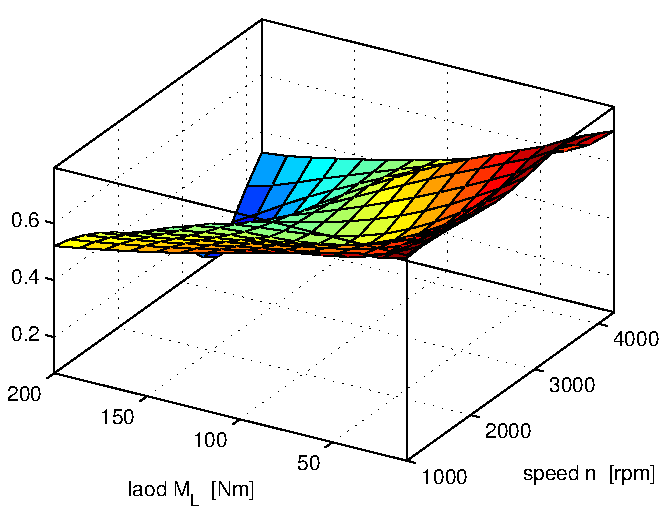
\includegraphics[width=0.75\textwidth]{images/k_surf.pdf}
   \caption{Ein Bild.}
   \label{fig:k_surf}
\end{figure}
\end{verbatim}

\begin{figure}
   \centering
   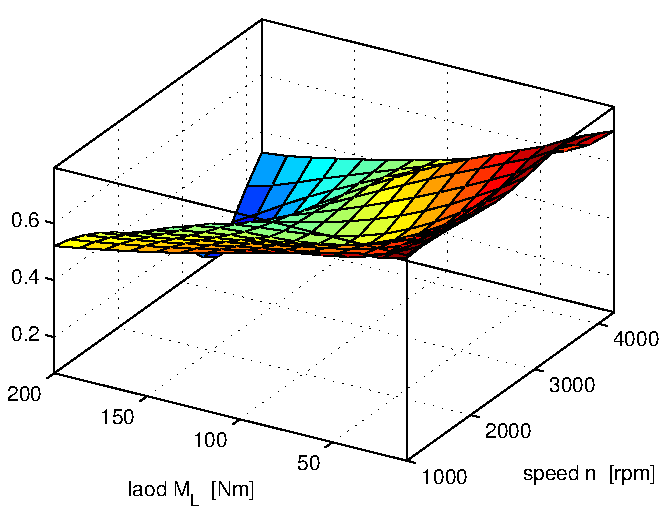
\includegraphics[width=0.75\textwidth]{images/k_surf.pdf}
   \caption{Ein Bild}
   \label{pics:k_surf}
\end{figure}

oder bei zwei Bildern nebeneinander mit:
\begin{verbatim}
\begin{figure}
  \begin{minipage}[t]{0.48\textwidth}
    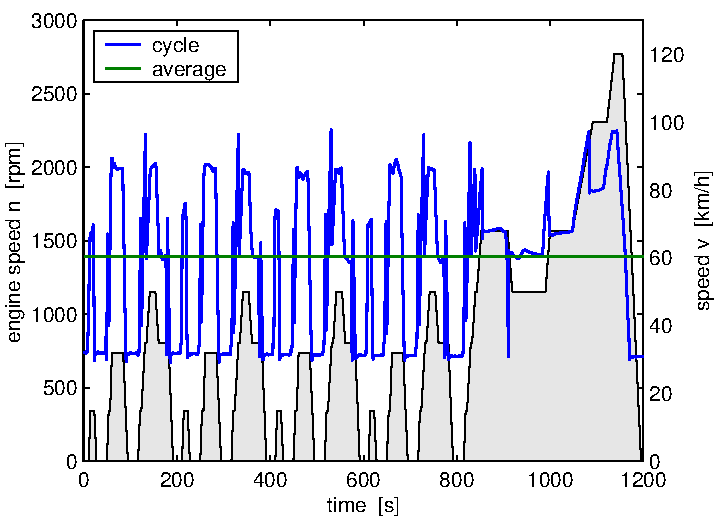
\includegraphics[width = \textwidth]{images/cycle_we.pdf}
  \end{minipage}
  \hfill
  \begin{minipage}[t]{0.48\textwidth}
    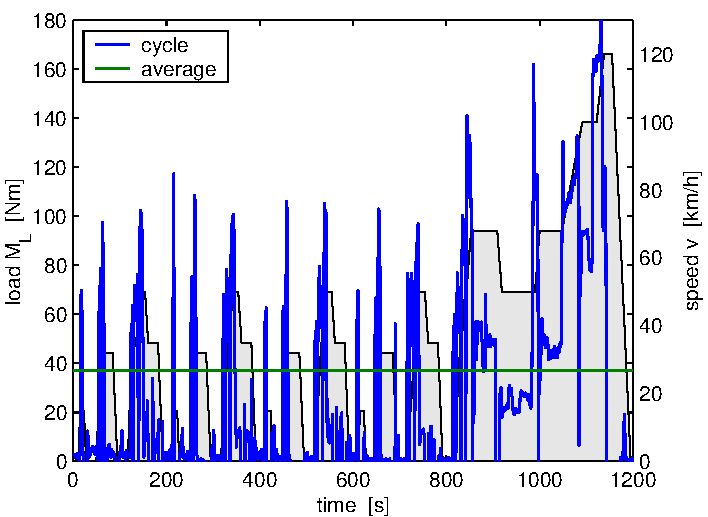
\includegraphics[width = \textwidth]{images/cycle_ml.pdf}
  \end{minipage}
  \caption{Zwei Bilder nebeneinander.}
  \label{pics:cycle}
\end{figure}
\end{verbatim}

\begin{figure}
  \begin{minipage}[t]{0.48\textwidth}
    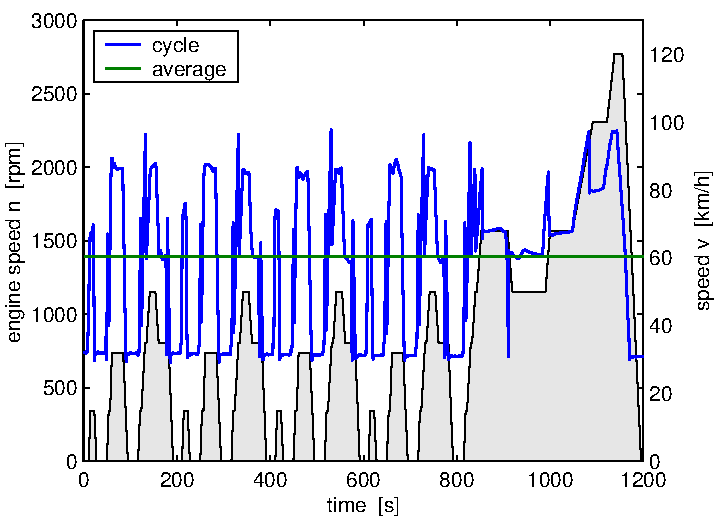
\includegraphics[width = \textwidth]{images/cycle_we.pdf}
  \end{minipage}
  \hfill
  \begin{minipage}[t]{0.48\textwidth}
    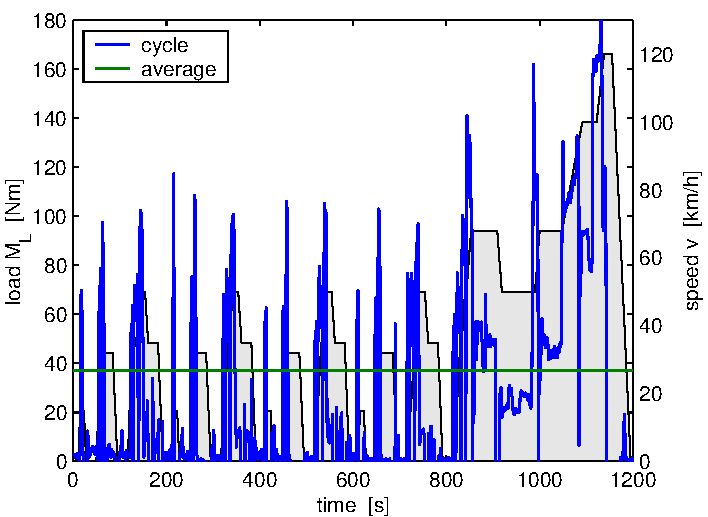
\includegraphics[width = \textwidth]{images/cycle_ml.pdf}
  \end{minipage}
  \caption{Zwei Bilder nebeneinander}
  \label{pics:cycle}
\end{figure}


\section{Mathematische Formeln}\label{sec:math}

Einfache mathematische Formeln werden mit der equation-Umgebung
erzeugt:
\begin{equation}
 p_{me0f}(T_e,\omega_e) \ = \ k_1(T_e) \cdot (k_2+k_3 S^2
 \omega_e^2) \cdot \Pi_{\mathrm{max}} \cdot \sqrt{\frac{k_4}{B}} \, .
 	\label{eq:my_equation}
\end{equation}

Der Code dazu lautet:
\begin{verbatim}
\begin{equation}
 p_{me0f}(T_e,\omega_e) \ = \ k_1(T_e) \cdot (k_2+k_3 S^2
 \omega_e^2) \cdot \Pi_{max} \cdot \sqrt{\frac{k_4}{B}} \, .
\end{equation}
\end{verbatim}

Mathematische Ausdrücke im Text werden mit \$formel\$ erzeugt (z.B.:
$a^2+b^2=c^2$).

Vektoren und Matrizen werden mit den Befehlen \texttt{\textbackslash vec\{.\}} und \texttt{\textbackslash mat\{.\}} erzeugt (z.B. $\vec{v}$, $\mat{M}$).


\section{Weitere nützliche Befehle}\label{sec:div}

Hervorhebungen im Text sehen so aus: \emph{hervorgehoben}. Erzeugt
werden sie mit dem \texttt{\textbackslash epmh\{.\}} Befehl.

Einheiten werden mit den Befehlen \texttt{\textbackslash unit[1]\{m\}} (z.B.~\unit[1]{m}) und \texttt{\textbackslash unitfrac[1]\{m\}\{s\}} (z.B.~\unitfrac[1]{m}{s}) gesetzt.


\chapter{Problem Definition}
\section{Vector Field Method}

There are different methods like Geometric, Nonlinear, Feedback linearlization, Optimal control, Model predictive control in the Path Following field.

However, Vector Field approach is the most extendable and simple for unifying the guidance output for the Hybrid VTOL use case. And thus was chosen as the basis for the formulation.

\section{Output of the Path Following Guidance}

The output of a vector field based path following guidance is a desired velocity vector. And the low level controller is expected to actuate the vehicle to achieve the desired velocity profile.

In some papers additional output like lateral acceleration, heading angle, etc are also formulated. However to simplify the application we do not constrain the guidance algorithm to also include any of those outputs.

\section{Constraints}
Here are the relevant constraints that a Path Following Guidance output should have:

\begin{enumerate}
    \item Holonomicity: Magnitude of the velocity curve should be holonomic while approaching the path
    \item Convergence time: Time it takes for a vehicle at a specified point to converge within specified distance to the path
    \item Acceleration: Acceleration required to follow the Vector Field
\end{enumerate}

\section{Terminology}

Here the relevant variables for the formulation of the methods are explained.

* Track error boundary
* Approach speed
* On-path speed

\begin{figure}[h]
\centering
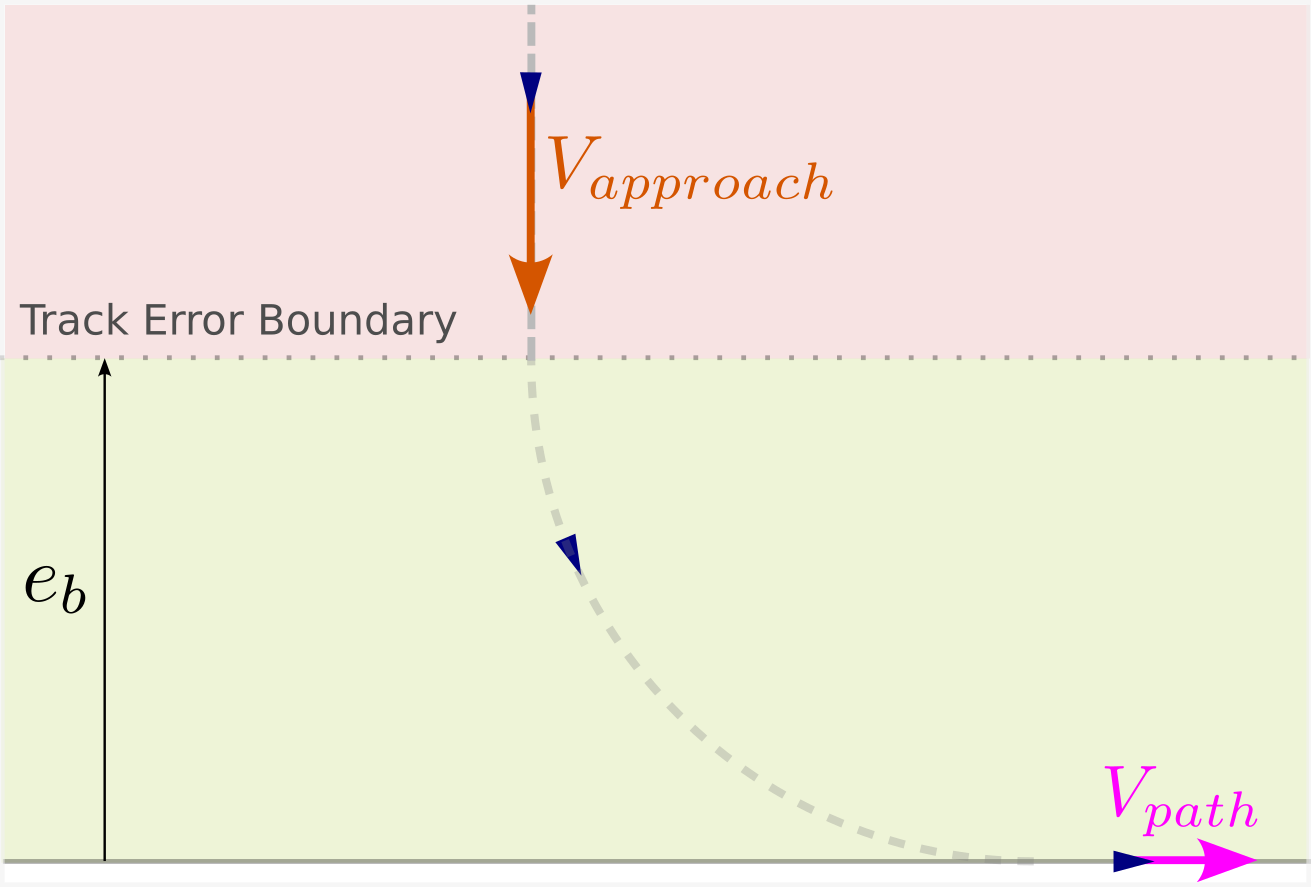
\includegraphics[width=\textwidth]{PathFollowing_Problem_v2_arrow_enlarged_simplified}
\caption{Path Following Problem Definition}
\end{figure}

\cleardoublepage

\chapter{Methods}
\section{Unicyclic}

As a base method to improve on, a Nonlinear Path Following Guidance for a Fixed Wing vehicle was chosen because the Fixed Wing presents the most conservative and constrained platform, and thus can be extended easily to incorporate more agile platform (e.g. Multirotor).

Since Fixed Wing has a relatively constant forward speed, the algorithm thus assumes a 'unicyclic' motion (i.e. As if we are steering a person riding a unicycle).

\begin{figure}[h]
\centering
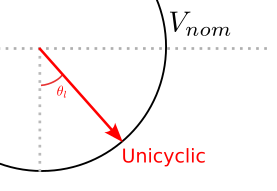
\includegraphics[width=0.7\textwidth]{Unicyclic_Formulation}
\caption{Unicyclic Formulation}
\end{figure}

** Explanation of the Unicyclic formulation

\section{Hybrid}

The presented formulation is noted as 'Hybrid', as it essentially is an adaptation of the Unicyclic formulation to account for a flexible velocity range  of a Multirotor.

\begin{figure}[h]
\centering
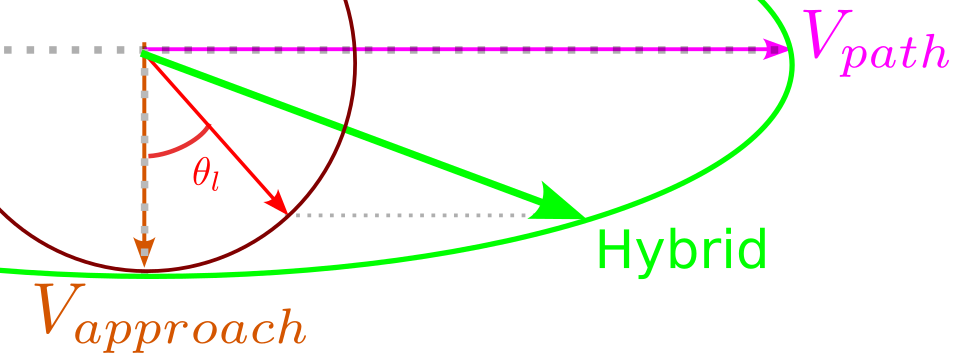
\includegraphics[width=0.7\textwidth]{Hybrid_Formulation}
\caption{Hybrid Formulation}
\end{figure}

** Explanation of the Hybrid formulation

\section{Maximum Acceleration}

This is a relaxed maximum acceleration (in path parallel, and orthogonal directions) calculation based vector field, where we assume that a vehicle approaching at $V_{approach}$ accelerates at highest possible acceleration to achieve $V_{path}$ while converging to the path.

% 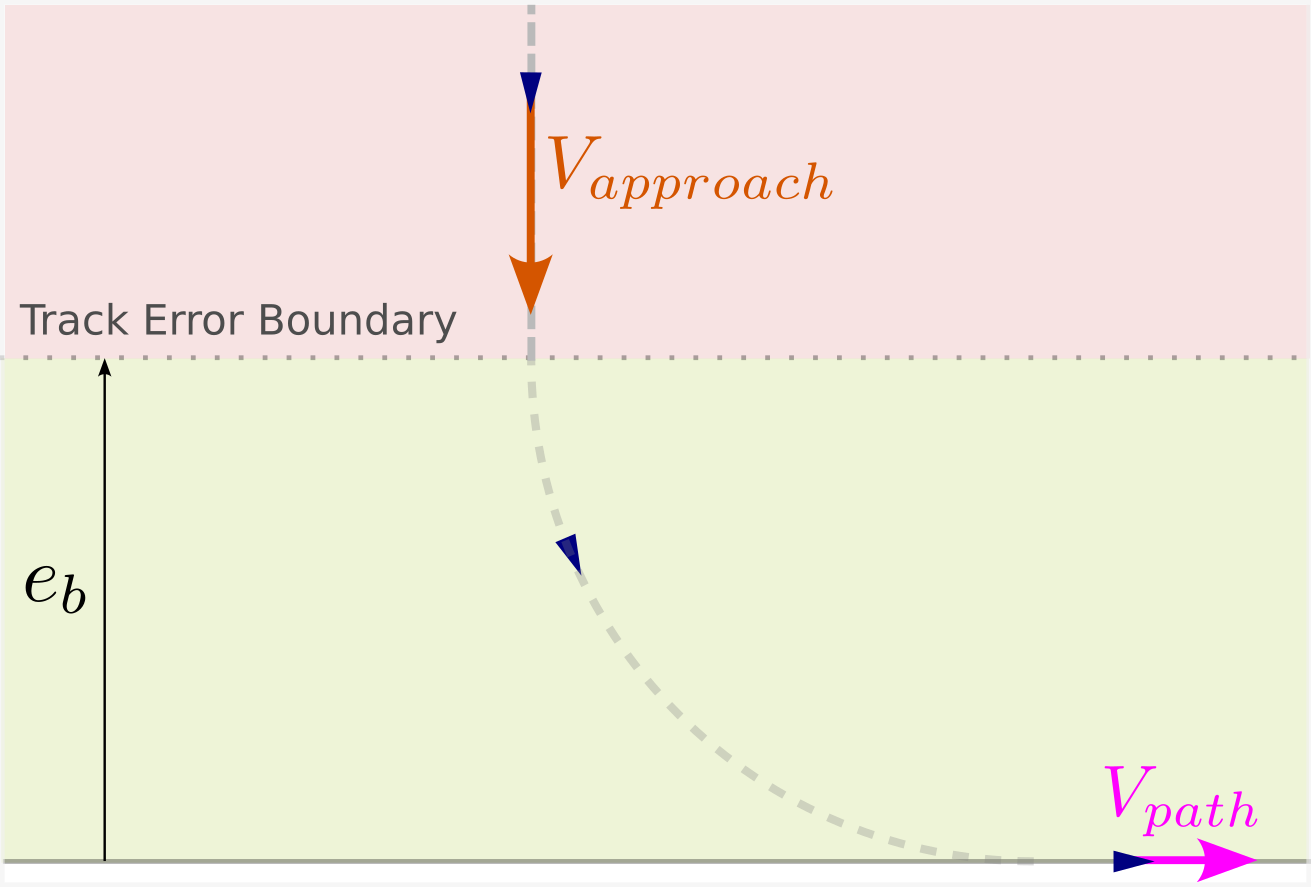
\includegraphics[width=\textwidth]{PathFollowing_Problem_v2_arrow_enlarged_simplified}

** Explanation of the Maximum Acceleration formulation

\cleardoublepage

\chapter{Evaluation}

\section{Approach \& On-path Velocity Constraint}

As expected, the $V_{approach}$ and $V_{path}$ is only expected in the Hybrid formulation.

\section{Low Speed On Path}

\includegraphics[width=0.7\textwidth]{VPath_0}

For a case where we desire to stop on the path, the hybrid formulation successfully demonstrates that it can approach the path orthogonally and come to a full stop.

\section{High Speed On Path}

\includegraphics[width=0.7\textwidth]{VPath_High}

For a high speed on path case, hybrid formulation shows a different approach geometry.

\section{Support For Fixed Wing Case}

As shown below, the Hybrid formulation still encompasses the unicyclic formulation as a special case, when the $V_{path} = V_{approach}$, which is designated as $V_{nom}$.

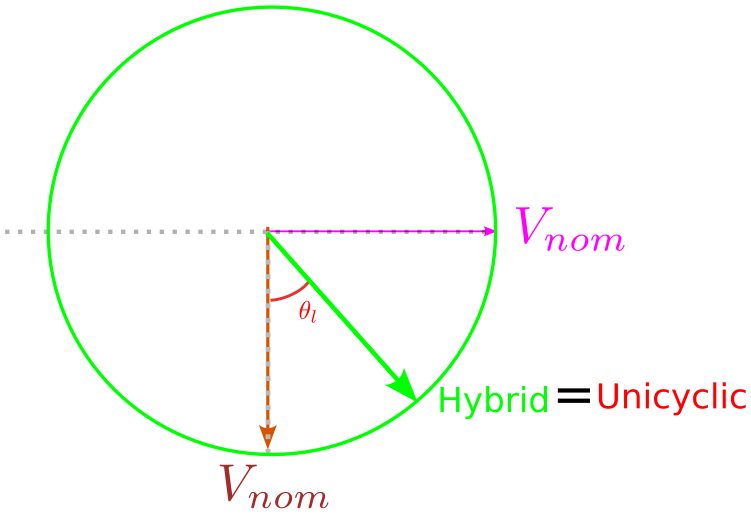
\includegraphics[width=0.7\textwidth]{Hybrid_Supporting_Unicyclic}

\cleardoublepage

\chapter{Conclusion \& Future Work}

This thesis successfully demonstrated that a unified guidance considering both Multirotor and Fixed Wing use cases for a Hybrid VTOL can be formulated.

The Hybrid formulation, as it was designed for satisfied the most number of constraints.

\section{Wind}
Since the acceleration constraint of a Fixed Wing is tied to it's yaw angle, which in turn is tied to the wind vector, it wasn't trivial to come up with a generic solution that would cover all the different wind cases in terms of the acceleration required by the Vector Field.

Therefore, it would be nice to incorporate wind more thoroughly in the guidance algorithm in the future for both Multirotor and Fixed Wing cases to create an actually optimal path following commands, and not just the ground velocity vector field.

\section{Low Level Control}
This thesis assumed that the low level controller would be capable of actuating the vehicle to track it's desired ground velocity. However, without the acceleration feed forward command directly computed from the spatial derivative of the Vector Field it would of course be challenging for the low level controller to tightly track the desired velocity.

Therefore, like done in the original unicyclic formulation, it is desirable to passthrough an actual acceleration command in body frame. 

\cleardoublepage

%%%%%%%%%%%%%%%%%%%%%%%%%%%%%%%%%%%%%%%%%%%%%%%%%%%%%%%%%%%%%%%%%%%%%%%%%%%%%%%
% Bibliography
%%%%%%%%%%%%%%%%%%%%%%%%%%%%%%%%%%%%%%%%%%%%%%%%%%%%%%%%%%%%%%%%%%%%%%%%%%%%%%%
% \bibliographystyle{bibliography/IEEEtranN}
% \bibliography{bibliography/references}
% \addcontentsline{toc}{chapter}{Bibliography}
% \cleardoublepage

%%%%%%%%%%%%%%%%%%%%%%%%%%%%%%%%%%%%%%%%%%%%%%%%%%%%%%%%%%%%%%%%%%%%%%%%%%%%%%%
% Appendix
%%%%%%%%%%%%%%%%%%%%%%%%%%%%%%%%%%%%%%%%%%%%%%%%%%%%%%%%%%%%%%%%%%%%%%%%%%%%%%%
% \appendix
% \chapter{Irgendwas}\label{sec:irgendwas}

Bla bla \dots
% \cleardoublepage
% \chapter{Datasheets}\label{sec:datasheets}

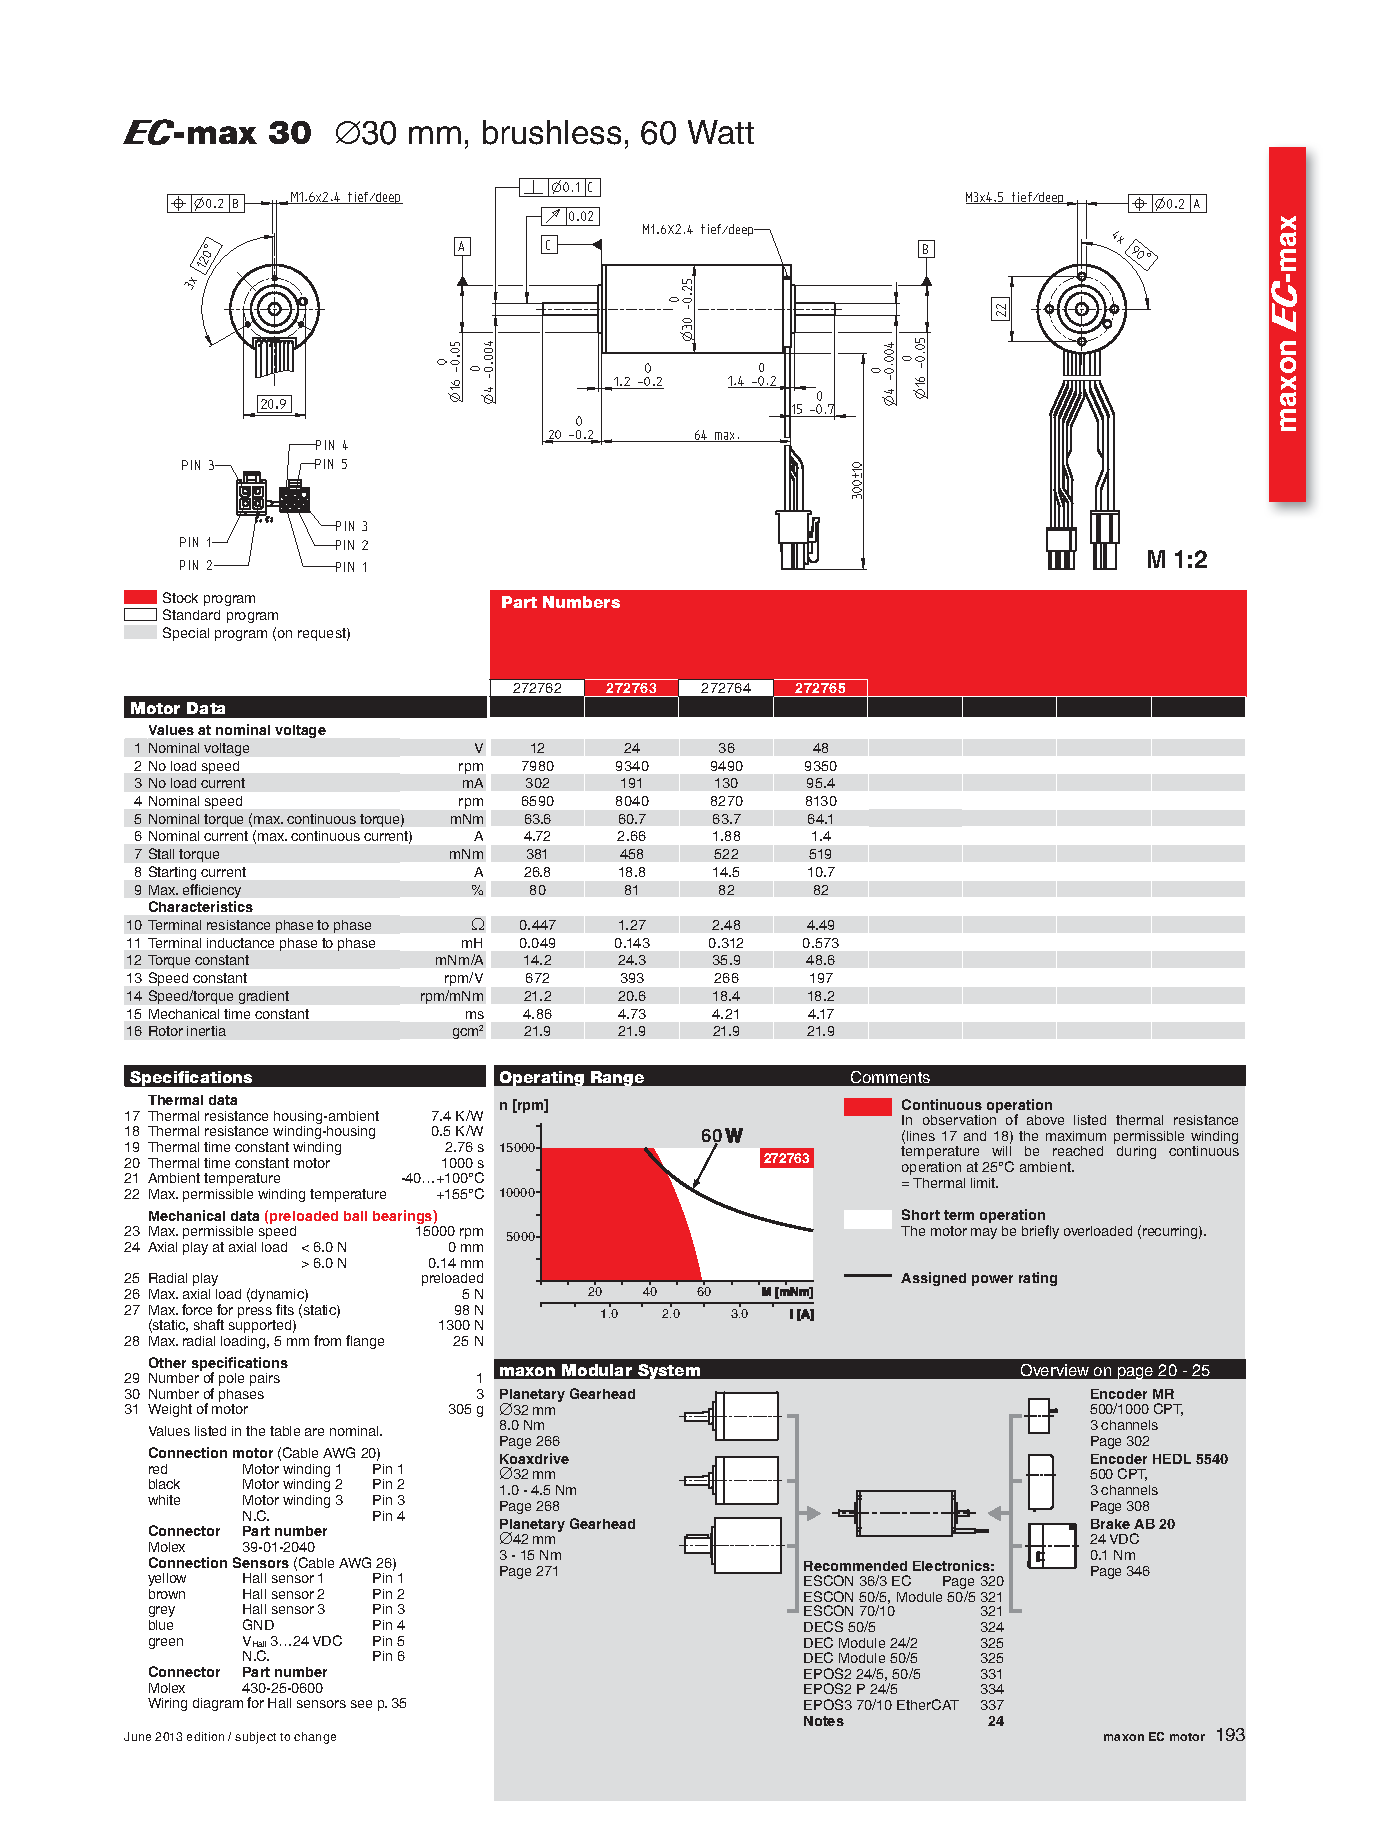
\includepdf[scale=0.75]{images/datasheets.pdf}

\end{document}